\documentclass[titlepage]{article}
\usepackage{adjustbox}
\usepackage{graphicx}
\graphicspath{ {./images/} }


%% DOCUMENT OUTLINE
% Cover Page
% Overview
% What sets the project apart?
% Story and gameplay
% Schedule

\title{Superhero Fantasy Platformer(working)\\
	\large Super Fantasy 7}
	%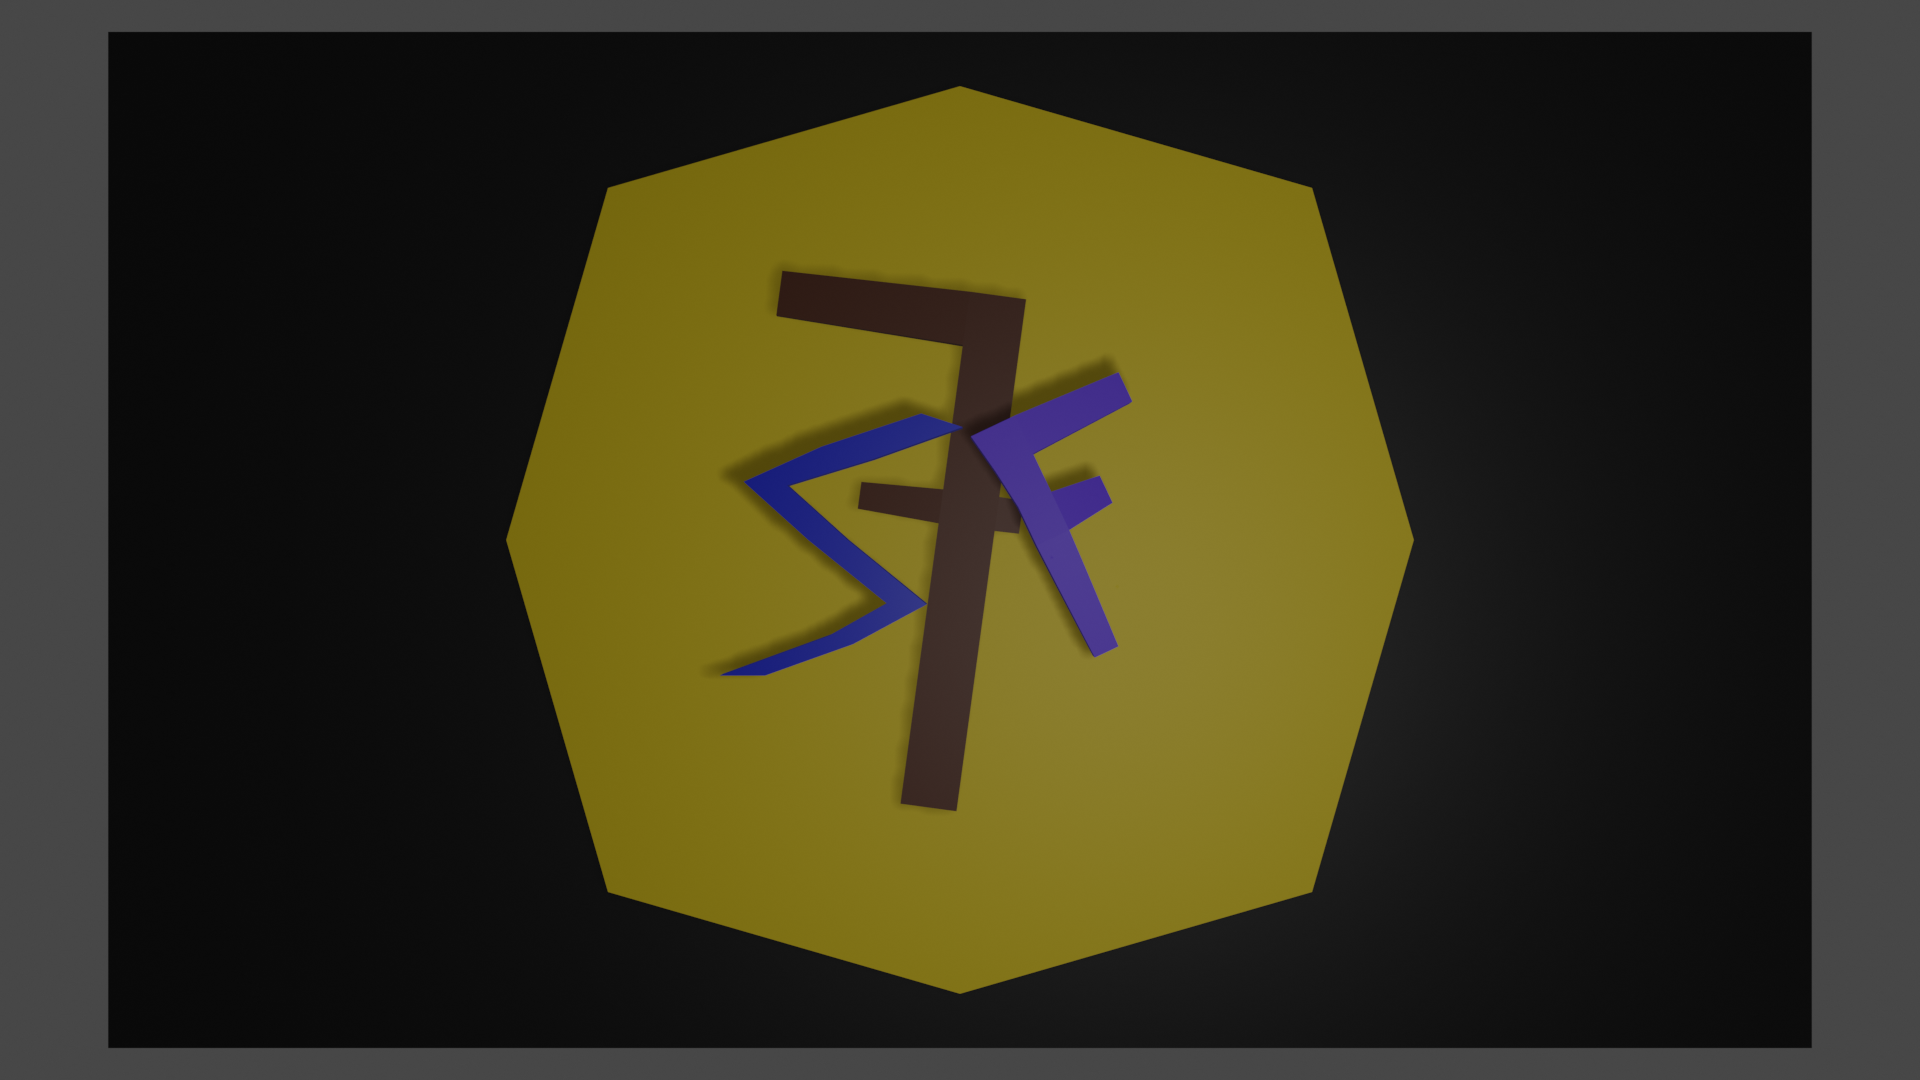
\includegraphics[scale=.15]{./images/logo.png}
	%for whatever reason, it will not appear here correctly
\author{Savanna Middaugh, Hannah Murphy, Orion Nassaux, Jacob Santillanes}
\date{\today\\v1.0.0}

\begin{document}
\maketitle
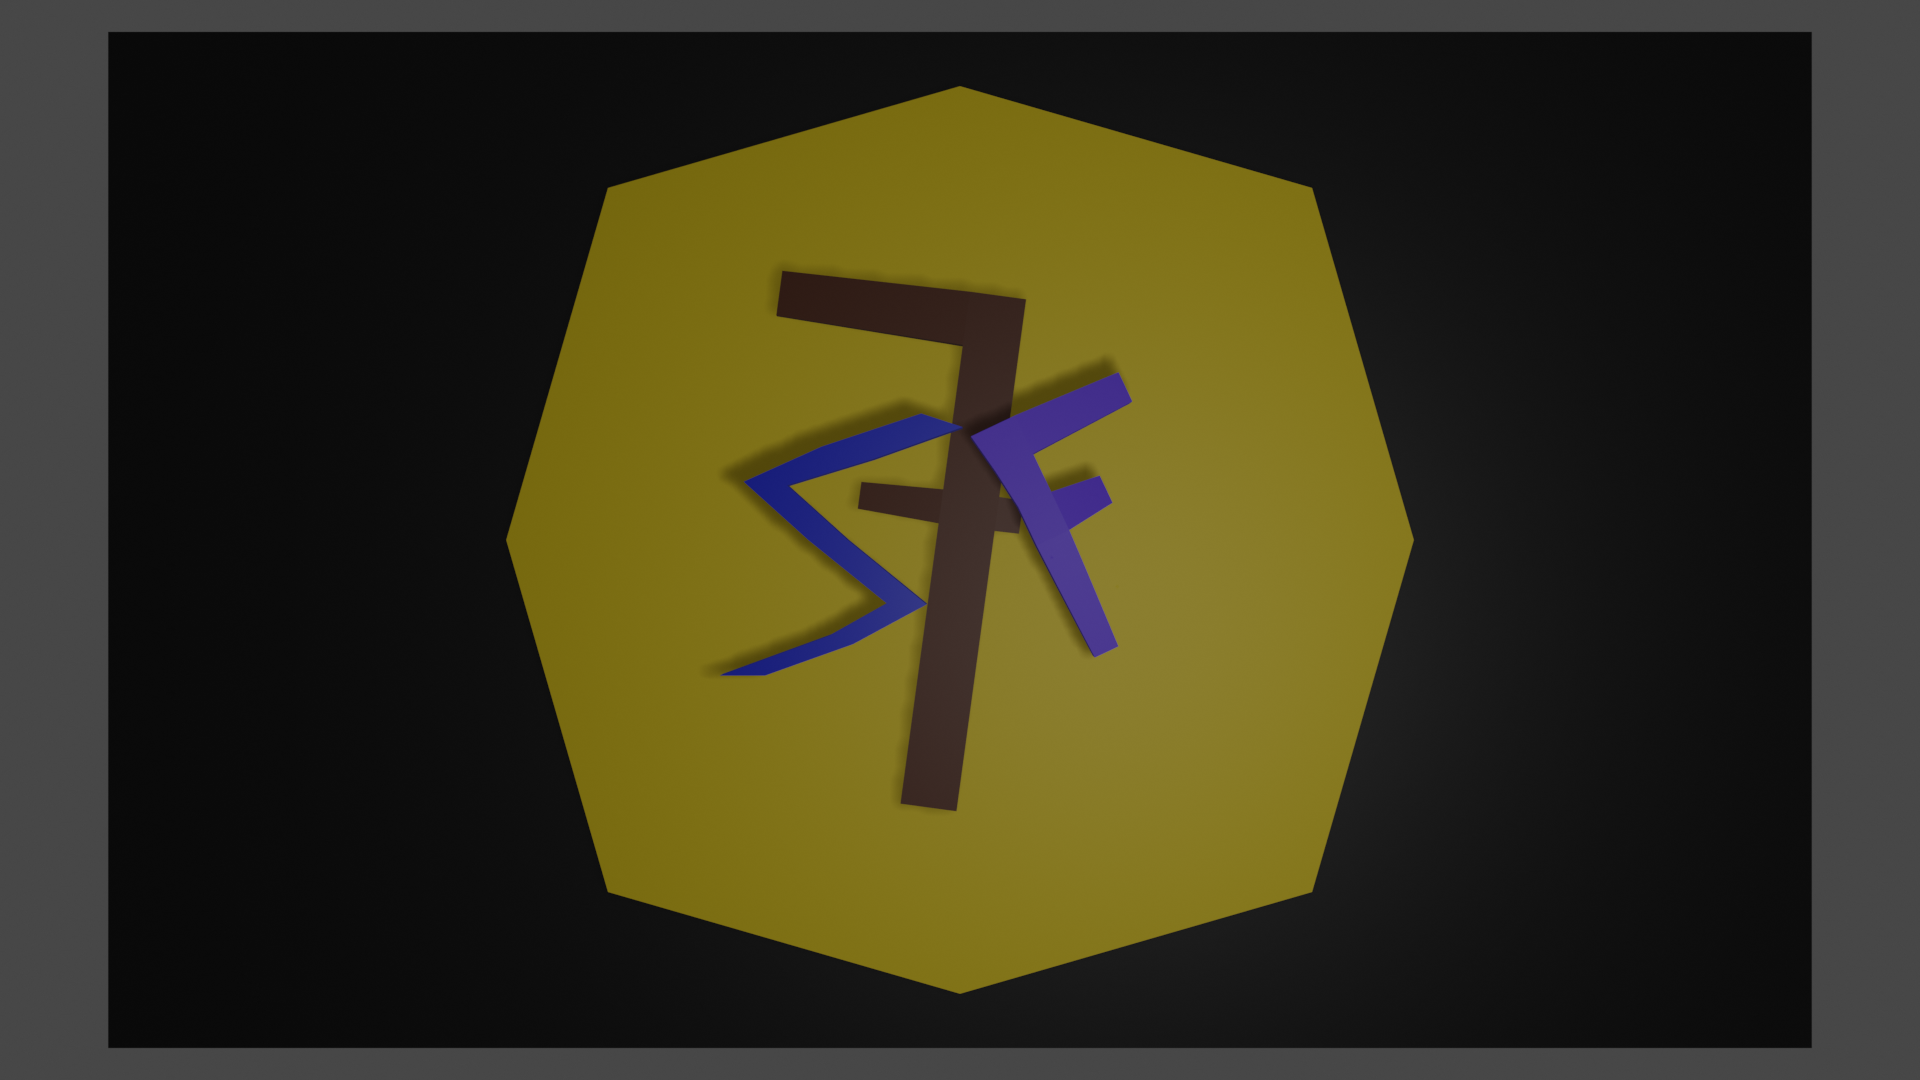
\includegraphics[scale=.15]{./images/logo.png}
%just so i can copy paste \subsection*{}
\section{Overview}

\subsection*{Theme, Setting, Genre}
We will be designing a 3d metroidvania platformer that takes place in a (mostly) renaissance medieval, high fantasy, setting. 

\subsection*{Core Gameplay Mechanics (Brief)}
The core gameplay will consist of going through dungeons to get a special item and killing the boss at the end of the dungeon. The dungeons will have at least two rooms with enemies and one puzzle room. The enemies you kill will drop health so as to keep the player playing aggressively rather than defensively. As you kill enemies you will get xp and you can use this to upgrade your skill with your items. 

\subsection*{Target Platform}
The game will be developed for PC using keyboard controls. Gamepad controllers will be implemented if time allows.

\subsection*{Project Scope}

\subsection*{Game Time Scale}
There will be a working version of this game at the end of the 16 week time frame that is given.

\subsection*{Team Structure}
Jacob Santillanes (Ulteelectrom) is in the art section of the class and will be proving assets for the game.
Savanna Middaugh (savymidd) will be providing assets for the game.
\subsection*{Licenses/Hardware/Other Info}
The game will be made in Unity with blender being used to create assests.  \\
Github repositiry: https://github.com/murphy-97/SuperFantasy7

\subsection*{Influences}
We took inspiration from several sources
\begin{itemize}
    \item Metroidvania games. We decided that this format was how we wanted to design the game play restrictions
    \item My Hero Academia, DC and Marvel comics: Superheroes are an element in the game.
    \item Fantasy Games (varied, like the Legend of Zelda games): We decided to go with a fantasy setting
    \item %Not sure where the skill tree idea came from
    \item Legend of Zelda games: the dungeons having a set pattern we can assume
    \item Rogue-like games: the dungeons having random rooms.
    \item %not sure where the item drop/health drop ideas came from
\end{itemize}
\subsection*{Elevator Pitch}
%I can't think of a good name - Orion
Dark lords stole the (placeholder name) causing the world to merge with another world. You have to defeat them and return the (placeholder name) to their rightful place in order to separate the worlds once again and return everything to normal. 

\section{Unique Project Aspects}
% Premise: sci-fi plus fantasy
% Dungeons: balance between random generation and prefab set pieces
\begin{itemize}
	\item Features a mix of both classic fantasy and superhero themes.
	\item Uses randomised dungeons to deliver a unique experience in every game.
\end{itemize}

\section{Story \& Gameplay}
% Two worlds collided when the magic thingies were stolen
% The player must defeat fantasy monsters and super villains to bring alignment back to the multiverse
\subsection*{Story (Brief)}
Bad Guys are merging two worlds together. One is a high fantasy setting and one is a super hero setting. You need to separate the worlds and return everything to normal. You play as either a hero or a knight. 

\subsection*{Gameplay (Brief)}
Basic platforming. The player can collect special items to interact with the environment or find new ways of beating the enemies. The player will have a basic attack, and a skill tree to upgrade their items and their basic attacks. 

\section{Schedule}
% Look at assignment due dates
% Start with two bosses and items
% Add a third boss and item if time
% Add a fourth boss and item if time

% 03 Feb: Conceptualization 2
% 10 Feb: Conceptualization 3
% 24 Feb: Pre-Production 1
% 26 Feb: Midterm!
% 02 Mar: Pre-Production 2
% 23 Mar: Production 1
% 30 Mar: Production 2
% 06 Apr: Production 3
% 13 Apr: Production 4
% 27 Apr: QA/Polish 1
% 01 May: QA/Polish 2

\end{document}

    